\documentclass{apa}

%\usepackage[utf8]{inputenc}
%\usepackage[american]{babel}

\usepackage{epsfig}
\usepackage{apacite}
\usepackage{graphicx}
\usepackage{bm}

\bibliographystyle{apacite}

% ---------- watermark -----------
\usepackage[firstpage]{draftwatermark}
\SetWatermarkAngle{0}
\SetWatermarkFontSize{0.25cm}
\SetWatermarkVerCenter{1.15cm}
\SetWatermarkLightness{0.5}
\SetWatermarkHorCenter{14cm}
\SetWatermarkText{\shortstack[l]{
Navarro, D. J. and Perfors, A. (2010). Similarity, feature discovery, \\
and the size principle. Acta Psychologica, 133, 256-268 \\
http://dx.doi.org/10.1016/j.actpsy.2009.10.008
}}
\SetWatermarkScale{1}
% -------------------------------



\newcommand{\s}{\eta}
\newcommand{\f}{f}
\newcommand{\be}{\begin{equation}}
\newcommand{\ee}{\end{equation}}

\newcommand{\presec}{\vspace*{6pt}}
\newcommand{\given}{\,|\,}
\newcommand{\follows}{\, \sim \,}
\newcommand{\mat}[1]{\mathbf{#1}}
\newcommand{\vct}[1]{\mathbf{#1}}
\newcommand{\exemplar}[1]{\textit{#1}}
\newcommand{\feature}[1]{\textsc{#1}}
\newcommand{\domain}[1]{\textsc{#1}}

\title{Similarity, feature discovery, and the size principle}

\twoauthors{\normalsize Danielle J. Navarro}{\normalsize Andrew Perfors}
\twoaffiliations{School of Psychology \\ University of Adelaide}{School of Psychology \\ University of Adelaide}
\rightheader{Generating and testing sparse hypotheses}
\shorttitle{Generating and testing sparse hypotheses}
\leftheader{Generating and testing sparse hypotheses}

\abstract{In this paper we consider the ``size principle'' for featural similarity, which states that rare features should be weighted more heavily than common features in people's evaluations of the similarity between two entities. Specifically, it predicts that if a feature is possessed by $n$ objects, the expected weight scales according to a $1/n$ law. One justification of the size principle emerges from a Bayesian analysis of simple induction problems (Tenenbaum \& Griffiths 2001), and is closely related to work by Shepard (1987) proposing universal laws for inductive generalization. In this article, we (1) show that the size principle can be more generally derived as an expression of a form of representational optimality, and (2) present analyses suggesting that across 11 different data sets in the domains of animals and artifacts, human judgments are in agreement with this law. A number of implications are discussed.}

\begin{document}
\maketitle

\section{Introduction}

Similarity offers a fundamental mechanism for organizing experience, imposing order on the ``great blooming, buzzing confusion'' \cite{James1890} presented to the senses. As a result, similarity data provide a powerful tool for understanding the kinds of mental representations that people use to make sense of their world.  Whether these mental representations are geometric \cite{Attneave1950,Torgerson1958}, hierarchical \cite{Sattath1977}, featural \cite{Tversky1977,Shepard1979} or structured in some other manner  \cite{Goldstone1994,Hahn2003}, they appear to provide powerful constraints on the kinds of inductive inferences that people draw in everyday life.
Nevertheless, much remains unknown about how people judge similarity, and many basic questions are still not fully understood. What characteristics of the world or of human cognition cause similarity to be organized the way that it is? How does similarity relate to the features possessed by objects, and what kinds of higher-order operations and structures are used to organize the features into coherent mental representations? These questions and many others form the basis of a considerable volume of current research.

Bound up with these questions about similarity are the unknowns associated with features themselves: what constitutes a feature and from where does it originate? These unknowns comprise at least three distinct issues:
\newcounter{lcount}
\begin{list}{\arabic{lcount}.}{\usecounter{lcount} \setlength{\itemsep}{3pt} \setlength{\itemindent}{0pt} \setlength{\listparindent}{6pt} }
\item {\it Feature discovery}. The feature discovery problem is the problem of extracting features from the ``blooming, buzzing confusion'' in the first place. If the world provides the learner with a large volume of noisy data to work with, how should he or she extract those features that approximate this information as simply as possible? Why, out of infinitely many possible features \cite{Goodman1955}, are certain {\em particular} features important? What are the rules that determine when the learner should propose that a feature actually exists? This problem has close ties to dimensionality reduction problems commonly studied in psychology and other disciplines \cite{Thurstone1947,Torgerson1958,Shepard1979,Navarro2008a}.
\item {\it Feature selection}. The feature selection problem is similar to the feature discovery problem, but is slightly simpler. Given that the learner has already chosen some features with which one can represent objects, how should he or she choose a subset of {\it relevant} features  that pertain to a particular problem? Although there is a high degree of variability when people are asked to list features, there is also substantial agreement, and feature lists have proven to be highly useful in understanding many aspects of human cognition, including conceptual structure, categorization, and semantic memory, among others \cite<see>[for a discussion]{McRaeetal2005}. This problem has strong ties to the theory of pragmatics and optimal communication in language \cite{Sperber1986,Frank2009}, and is discussed in some detail by \citeA{Zeigenfuse2009} in this volume.
\item {\it Feature weighting}. How much importance should be attached to any particular feature in any particular context? When trying to determine how similar two objects are, which features are more likely to provide the relevant {\it respects} for similarity \cite{Medinetal1993}, and how is this determined? This issue has strong ties to the Bayesian theory of generalization \cite{Tenenbaum2001,Sanjana2002,Navarro2008b}, which we discuss later.
\end{list}

\noindent
Note that these three issues overlap to some extent: feature weighting and selection could be treated as a single problem if weights of zero are allowed, and feature discovery can be thought of as the most difficult type of feature selection, in which every logically possible feature is considered as a possible candidate for inclusion. However, each issue focuses on different problems, so these distinctions are still helpful.

Recent work in the Bayesian framework has proposed a general {\it size principle} for cognition \cite<e.g.,>{Tenenbaum2001,Sanjana2002,Xu2007,Navarro2008b,Frank2009}. In the context of features and similarities, the size principle predicts a relationship between the ``size'' of a feature's extension (i.e., the number of objects possessing it) and the extent to which objects that possess it are similar to each other. A general feature such as \feature{is a thing} has an extremely large extension, picking out all members of the class \domain{things}, whereas a specific feature such as \feature{has a prehensile tail} is narrower, picking out only things like \domain{monkeys}. In most papers, the origin of the size principle relates to the implicit sampling assumptions in the feature weighting problem \cite{Tenenbaum2001}, though some authors have considered the role of information communication in selection problems \cite{Frank2009}.

This paper is split into three main parts. In the first, we review some necessary background and describe how the analysis of \citeA{Tenenbaum2001} produces the size principle during {\it feature weighting} and the assumptions on which the analysis relies. In the second part to the paper, we discuss and expand on the {\it feature selection} based analysis of \citeA{Frank2009},  allowing us to derive the size principle from the {\it feature discovery} problem. We show that as a natural consequence of the central limit theorem, a learner who seeks to encode the world using  a small number of coherent features will converge on a mental representation of similarity that weights smaller reference classes more highly. In the third part of the paper, having motivated the size principle from these different perspectives, we then put it to a strong empirical test by evaluating it on the Leuven dataset of objects and features in 11 different domains.  We conclude with a discussion of the implications of the different analyses.

\section{Sampling Assumptions and the Size Principle}

Before beginning our derivation of the size principle for similarity, some background is necessary. We first describe a simple model that relates features to similarity, and then explain how the analysis of \citeA{Tenenbaum2001} extends this model, deriving the size principle based on certain assumptions about how objects are sampled from the world. This forms the background for understanding our analysis, which is presented in part two of the paper.

\subsection{The common features model: Simple but useful}


The Bayesian model described in this paper is based on the familiar common features model \cite{Tversky1977,Shepard1979} in which the assessment of the similarity $s_{ij}$ between two entities $x_i$ and $x_j$ depends only on those features they share. That is,
\begin{equation}
s_{ij} \approx \sum_k f_{ik} f_{jk} w_k,
\label{cf}
\end{equation}
\noindent
where $f_{ik}=1$ if the entity $x_i$ possesses the $k$-th feature, $f_{ik}=0$ if it does not, and $w_k$ is a non-negative saliency weight associated with the feature. This resemblance is a consequence of some deliberate simplifications we made in constructing our analysis, and should not be taken as a strong commitment to the common features model. We therefore address some of the shortfalls of the common features model in order to reassure the reader that they do not present a difficulty for our analysis.

The most obvious shortfall with the common features model is the fact that it relies strongly on  features, defined as ``binary indicator variables used to pick out groups of similar entities.'' In some domains, binary assignments do not provide a good approximation to the underlying stimulus representation \cite{Tversky1986}, and it is better to use continuous-valued stimulus dimensions instead. In some cases, it is necessary to use both kinds of representations together \cite{Navarro2003}. Additionally, there are situations where a featural model can represent the domain but is less parsimonious than a more structured approach \cite{Goldstone1994}. In this paper we consider cases where participants actually provided explicit lists of binary features; in such cases, a pragmatic reliance on featural representations does not seem inappropriate.

A second issue relates to the particular way in which featural similarity is defined in the common features model: similarity is assumed to be symmetric (in the sense that $s_{ij} = s_{ji}$), an assumption that is frequently violated in empirical data. While this is a legitimate issue with common features models, it does not matter for the current analysis since the data sets that we consider are all symmetric by experimental design. Alternatively, it would be a problem if Bayesian similarity models were fundamentally incapable of representing asymmetric similarity relations. Fortunately, this is not the case: it is fairly easy to derive asymmetric models such as the ratio model \cite{Gregson1975,Tversky1977} from basic probabilistic assumptions. \citeA{Tenenbaum2001} provide one such derivation, though others are possible.

A third issue is the related concern of incompleteness. Without additional assumptions about information retrieval \cite<e.g.,>[ch. 6]{Navarro2003c}, the
common features model makes no predictions about the time-course of similarity judgment or the sequence of mental operations that support it, whereas other models are able to capture a number of basic phenomena in this respect \cite{Goldstone1994,Hahn2003}. Along similar lines, the common features model treats all features as essentially being of the same type, making no distinction between the perceptual characteristics of a \exemplar{tiger} (e.g., \feature{is orange}), its category memberships (e.g., \feature{is a carnivore}), and its more abstract semantic associations (e.g., \feature{is associated with the Weeroona Bay football club}). All such characteristics are treated as ``features'', since they supply a respect in which two entities may be similar. Since the common features model is incapable of representing such distinctions, it is incomplete in a fundamental sense. However, it is important to recognize that while this kind of incompleteness means that the common features model cannot be a sufficient explanation for subjective similarity, it does not have any obvious bearing on the question at hand, which is to ask whether there exists any systematic relationship between the number of entities possessing a feature and the importance attached to it.


\subsection{Expansion of the common features model to incorporate sampling}

In this subsection we demonstrate how the common features model can be extended to incorporate sampling assumptions. The result is a slight variation on the generalization model described in \citeA{Tenenbaum2001}.

Let $\mathcal{X}=(x_1,\ldots,x_n)$ denote the set of entities in the domain, and let $\mathcal{C}=(c_1, \ldots, c_m)$ denote a collection of domain-relevant consequential sets, or classes. These sets represent the learner's hypotheses for why entities should be treated similar to one another in this context; when asked ``are \exemplar{apples} and \exemplar{tennis balls} similar?'' the answer would be ``yes'' if the relevant attribute is shape, and ``no'' if it is edibility. That is, our learner assumes that one of the consequential sets $c^*$ provides the relevant respect for similarity.\footnote{It is possible to extend this to multiple-respect models in a straightforward way, by allowing disjunctive hypotheses to be formed from the ``primitive'' set, allowing \feature{either round or green} and \feature{round and green} to be incorporated. This kind of composite hypothesis space has been considered by several authors \cite<e.g.,>{Goodman2008,Tenenbaum2001a,Sanjana2002,Navarro2006}. Here we are primarily interested in those features listed by people and thus avoid looking at possible combinations of those features unless such combinations were themselves explicitly listed. In any case, the form of the model can still be written as a weighted additive function -- the sum is simply taken over a much larger set of candidates.}

In light of these assumptions, what information is made available to the learner by the statement ``$x_i$ and $x_j$ are similar''? This statement explicitly asserts that $x_i$ and $x_j$ are both in some consequential set or class $c^*$ (formally, that $(x_i, x_j) \in c^*$ for some unstated set $c^* \in \mathcal{C}$). In addition, the statement {\it selects} the entities $x_i$ and $x_j$ for comparison; if the selection process is influenced by the kinds of regularities $\mathcal{C}$ present in the domain, then this can convey information about the nature of $c^*$. If we let $s_{ij}$ denote the similarity of $x_i$ and $x_j$, we obtain
\begin{eqnarray}
s_{ij} &=& \Pr(x_i \in c^*,x_j \in c^*,x_i,x_j \given x_i \in \mathcal{X}, x_j \in \mathcal{X}, c^*\in \mathcal{C}) \\
&=& \sum_{k=1}^m \Pr(x_i, x_j, x_i \in c_k, x_j \in c_k \given x_i \in \mathcal{X}, x_j \in \mathcal{X}, c^* = c_k) \Pr(c^* = c_k \given c^* \in \mathcal{C}),
\end{eqnarray}
\noindent
where there are $m$ possible consequential sets and the summation in the second line expresses the uncertainty about which element $c^*$ is the relevant one for the statement. If we take the $x \in \mathcal{X}$ and $c\in \mathcal{C}$ conditions as given, and assume that the four pieces of information in the similarity statement are exchangeable, then
\begin{eqnarray}
s_{ij} &=& \sum_{k=1}^m \Pr(x_i\in c_k, x_j \in c_k \given x_i, x_j, c_k) \Pr(x_i,x_j \given c_k) \Pr(c_k) \\
&=& \sum_{k=1}^m z_{ik} z_{jk}  \Pr(x_i,x_j \given c_k)  \Pr(c_k),
\end{eqnarray}
\noindent
where $z_{ik}$ denotes whether item $x_i$ is in class $k$ (i.e., $z_{ik} = 1$ if $x_i \in c_k$ and 0 otherwise). The $\Pr(c_k)$ term describes the prior probability that the relevant class $c^*$ is in fact $c_k$, and for the current purposes we assume that this is a fairly arbitrary weighting function.\footnote{The way to derive the ratio model is for the learner to assume that $c^*$ is not randomly selected from $\mathcal{C}$, but rather is drawn from a restricted set $\mathcal{C}^-$ that only includes those sets $c$ such that $x_i \in c$ or $x_j \in c$. This assumption makes sense in some contexts, but we do not pursue it here.} Accordingly, letting $\Pr(c_k) \propto w_k$ denote this function, and assuming that the consequential sets $\mathcal{C}$ correspond to classes of entities that share some feature (i.e., $z_{ik} \equiv f_{ik}$), then
\begin{equation}
s_{ij} = \sum_{k=1}^{m} f_{ik} f_{jk} w_k \Pr(x_i, x_j \given c_k).
\end{equation}

We now have an expression that is equivalent to the common features model (Equation~\ref{cf}) except for the additional term $\Pr(x_i,x_j \given c_k)$. It is this $\Pr(x_i, x_j \given c_k)$ term that is of most interest to us here. This term refers to the manner in which the items $x_i$ and $x_j$ are sampled -- the manner in which they are assumed (by the learner) to have been generated (by the speaker or world). We consider possible ways of calculating this in the next section, and show that the size principle for similarity emerges as a consequence of one particular sampling assumption.

\subsection{Strong sampling and the size principle}

In most similarity experiments, the actual process by which the query items are generated is obvious: the experimenter systematically asks about all possible pairs of distinct entities in $\mathcal{X}$, and so the probability of observing the pair $(x_i, x_j)$ is entirely independent of $c^*$. However, this is not particularly representative of how similarity works in real life, where similarities are either spontaneously noticed among the objects that one happens to encounter (which is generally non-random), or are suggested in conversation (also generally non-random). People are much more likely to spontaneously notice that \exemplar{birds} are like \exemplar{bats} when the topic of conversation involves \feature{things that can fly} than in the context of conversations about a more general topic \feature{things that breathe}, much less the totally irrelevant topic \feature{18th century astrophysics}. If people apply natural sampling assumptions, then the mere fact of having been asked about \exemplar{birds} and \exemplar{bats} is evidence that the relevant respect for similarity is more likely to be \feature{things that can fly} than either \feature{things that breathe} or \feature{things relevant to 18th century astrophysics}.

To formalize this, we can consider a number of possibilities for $\Pr(x_i, x_j \given c_k)$. The exhaustive listing method used in experiments is an example of {\it weak sampling}, in which the observed entities are generated independently of the consequential set $c_k$. If, for simplicity, an entity is sampled uniformly from $\mathcal{X}$, we get\footnote{To be precise, $\Pr(x_i \given c_k) = 1/{|\mathcal{X}|}$, where $|\mathcal{X}|$ is the number of objects in $\mathcal{X}$. In other words, the probability of observing object $x_i$ is proportional to the number of objects in the domain.  Crucially, it does not depend on the size of the consequential set $c_k$.}
\begin{equation}
\Pr(x_i \given c_k) \propto 1.
\end{equation}
That is, the object $x_i$ is observed as a result of some process that does not in any way depend on the consequential set, or class, $c_k$. This sampling scheme was used by \citeA{Shepard1987} when formalizing his exponential law of generalization.  Alternatively, \citeA{Tenenbaum2001} proposed that in some contexts it is more appropriate to assume a {\it strong sampling} scheme in which items are sampled explicitly from the relevant class. If an observation is generated in this fashion, we obtain
\begin{equation}
\Pr(x_i\given c_k) = \left\{ \begin{array}{cl} 1/{n_k} & \mbox{ if } x_i \in c_k \\ 0 & \mbox{ otherwise} \end{array} \right.,
\end{equation}
\noindent
where $n_k = |c_k|$ denotes the number of entities belonging to the class (i.e., its size). If one wanted to judge the similarity between two items $x_i$ and $x_j$, one would need to evaluate it with respect to all possible classes; as a result of strong sampling, smaller classes that contain both $x_i$ and $x_j$ would assign higher probability to the data, and should therefore be expected to be weighted more heavily in people's similarity judgments than larger classes. This is the size principle for similarity as derived by \citeA{Tenenbaum2001}.\footnote{If both $x_i$ and $x_j$ are sampled from the consequential set, then the weighting term would be $\Pr(x_i, x_j \given c_k) = 1/{n_k}^2$. However, \citeA{Tenenbaum2001} argued for a sampling scheme based on the idea that only {\it one} of the entities was known to have been sampled from $c_k$ and the question at issue was whether having observed (say) $x_i$, some property would generalize to item $x_j$. With only one item known to belong to the class, the weighting factor for a similarity judgment would take the form of a $1/n_k$ rule rather than a $1/{n_k}^2$ rule. There is a strong pragmatic basis for this claim: if the learner knows in advance that both entities are drawn from the class, then he or she can state categorically that they are similar in the relevant respect, even if they cannot say what it is (and hence $s_{ij}=1$ for all $i$ and $j$). This is unlikely to be true of most contexts.}

As long as such classes are ``Type I'' categories in the \citeA{Shepard1961} sense\footnote{Technically, as long as a disjunction or conjunction of features can be said to produce a consequential set, then we need not restrict ourselves to ``Type I" categories. However, the restriction is convenient, since Type I categories correspond to salient regularities in people's mental representations \cite{Shepard1961}.}, any class is effectively equivalent to a feature -- the class of \feature{things that eat peanuts} indexes the same entities as those that share the feature \feature{eats peanuts}, and so on. Thus, the size principle is in fact a statement about the sort of features that will be weighted highly by a rational learner who assumes strong sampling: the smaller a feature is -- the fewer entities that share that feature -- the more important it should be.

\section{On the Origins of Features}

So far we have seen how the size principle for similarity judgment emerges naturally from an assumption that objects are strongly sampled from the world. In contexts in which a person has to compare two objects and determine how similar they are, strong sampling seems like a reasonable assumption.  This is particularly true when the objects are obviously sampled in a certain way, as in experimental or conversational situations in which the context explicitly constrains the consequential sets from which the objects are chosen. Although it is difficult to say for sure, it seems plausible to think that sampling done ``by the world'' is at the very least non-random, and may (at least sometimes) more closely resemble strong sampling than any other.

However, there are also circumstances in which strong sampling assumptions obviously do not hold. For instance, one obvious instance of weak sampling is the standard experimental paradigm for similarity, in which the experimenter systematically queries the participant about all possible pairs of distinct entities. To the extent that similarity data show a size effect (as illustrated later) when collected in this manner, something is amiss. One possibility is that people have an intuitive bias to assume that objects in real life are strongly sampled, which leads them to reject the artificial nature of the ``exhaustive pairwise sampling'' method.
While there is probably some truth to this, it is not an entirely satisfying explanation. For instance, in a somewhat different inductive generalization task, \citeA{Navarro2008b} sought to infer the sampling assumptions made by participants by using a model that smoothly interpolated between strong and weak sampling. The results suggested that the majority of people used a fairly weak sampling model, with a significant minority of participants applying stronger sampling assumptions. It may be that people make fundamentally different assumptions about the origins of data when switching from a feature induction task to a similarity judgment task, but this seems unlikely.

There is another, more fundamental, issue at play here as well. While it is useful to have some notion about how features are weighted in the context of similarity judgment tasks, there is a sense in which the underlying problem is considerably more general. Put simply, it is not only the case that people need to weight features when making judgments \cite<as per>{Tenenbaum2001} or select a single most-informative word to describe an object \cite<as per>{Frank2009}. Before any such action is possible, we need to discover or extract a set of useful features in the first place. In what follows, we demonstrate that the feature discovery problem itself induces a size principle.

\subsection{Size effects in feature discovery: The derivation from central limits}

To motivate our approach it is instructive to consider the derivation presented by \citeA{Frank2009}. As in \citeA{Tenenbaum2001}, they associate the $k$-th consequential set (in their case a set of possible word referents) with a uniform distribution over $n_k$ entities, but they make somewhat different assumptions about where the consequential set comes from.  \citeA{Tenenbaum2001} assume that the world selects the true class more or less randomly, and then generates observations from that class. The learner then seeks to identify the class using the information conveyed by the sampling process. In contrast, in \citeA{Frank2009} the world picks the observation more or less at random, and the learner specifies a class that would be maximally informative about that observation. Not surprisingly, the two yield equivalent results: the learner should try to specify the most specific word or smallest set that is consistent with the observation. For our purposes the interesting thing is not the specific result per se, but the weakened assumptions that produced it: namely, the fact that there is no need for the observation to be strongly sampled, only that the consequential set be informative.

In this section, we extend the approach taken by \citeA{Frank2009}, and propose that the size principle for similarity need not be a consequence of the sampling assumptions that generate objects at all. All that is required is that the underlying mental representations be chosen to optimally encode some structure in the world. One manner in which this can occur is equivalent to the \citeA{Frank2009} situation in which people select, from among the features in their mental representation, those that are most informative as to the underlying similarities between entities. However, our derivation is much more general, and does not require any pre-existing feature set at all -- the law arises naturally from the {\it feature discovery} process, in which the learner is assumed to extract a collection of features that encode some structure in the world. The nice thing about this approach is that it is able to explain why the size principle is able to emerge even when strong sampling seems to be violated. Later in the paper we put this prediction to the test. For now, however, we only derive and explain it. Why should rational feature discovery result in weighting smaller features more highly, according to a $1/n$ law?

Consider the simplest possible case, in which the world provides the learner with some resemblance structure. We denote that structure with $\mathbf{\Omega}=[\omega_{ij}]$ and imagine that it captures something like the ``true'' similarity matrix provided by the environment.\footnote{This is to be contrasted with the similarity inferred by the learner, which we denote throughout the paper as $s_{ij}$. That said, one special case of the framework arises when the learner attempts to select an informative subset of their pre-existing mental representation for a feature listing task, in which case the learner deliberately uses their own subjective similarities $\mathbf{S}$ in place of $\mathbf{\Omega}$. Roughly speaking, this corresponds to the assumption that feature listing is maximally informative, as in \citeA{Frank2009}, though the analogy is not quite exact.} Such a structure might be produced by a  large number of low-weight ``microfeatures'' observable in the environment; in such a case, $\omega_{ij}$ simply denotes the proportion of such features that are shared by two stimuli. However, the exact origin of this knowledge is irrelevant to our purposes; it only matters that it exists. Having observed this structure $\mathbf{\Omega}$ through experience, people need to extract a smallish number of more sensible features $\mat{F}$, a set of associated weights $\vct{w}$, and the inferred similarities $s_{ij}$. We do not assume that the features are re-weighted further when assessed in contexts that require the judgment of similarity. Formally, this means we assume that $s_{ij} \approx \sum_k f_{ik} f_{ik} w_k$, as per the original common features model (Equation~\ref{cf}). In other words, to the extent that there are any systematic biases among the weights of different features, our analysis assumes that they arise in the initial learning of $\mat{F}$ and $\vct{w}$.

What is the nature of $\mathbf{\Omega}$? On the one hand, it is quite clear that the real world has a great deal of structure; to give just one example, we know that perceptual representations are highly structured, likely as a result of specific evolutionary pressures.  It is also apparent that direct experience of the world is not the only way that information is made available to people: we learn pedagogically and vicariously as well. These points are not a concern to our analysis, since we are not proposing a complete model for learning nor do we care (for now) about the precise knowledge that comprises $\mathbf{\Omega}$. Rather, we are attempting to show that -- all else being equal -- a learner seeking to represent the structure of the world using a smallish collection of features will end up with a size principle, weighting the features that index fewer entities in the world more highly. In support of this proposition, we consider the extreme case where $\mathbf{\Omega}$ is entirely arbitrary. In that case, that the information available to the learner would reflect only the simple fact that some things are similar, and other things are not. Our point is that {\it on this basis alone}, a size principle emerges. Naturally, if the world provides a {\it particular} structure that implies a different law, then other laws might emerge. However, if the world provides no bias, then a rational learner should supply one, and the supplied bias takes the form of a $1/n$ law.

If the goal is to encode the resemblance structure of this world $\mathbf{\Omega}$ as effectively as possible, which features should the learner include in their mental representation? Intuitively, an effective feature should pick out a {\it coherent} subset of entities -- those entities that are highly similar to one another. If some feature is possessed by $n=|c|$ entities, then we need to calculate the average similarity $\bar{\omega}$, taken over all $N=n(n-1)/2$ pairs of entities that share the feature.  In our minimally structured environment, we assume that the ``true'' similarities $\omega_{ij}$ are randomly generated from some unknown distribution that has finite mean $\mu$ and variance $\sigma^2$. If so, then the central limit theorem \cite<e.g.,>[theorem B.97]{Schervish1995} implies that
\begin{equation}
\lim_{N \rightarrow \infty} \sqrt{N} (\bar{\omega} - \mu) \rightarrow \mbox{Normal}(0,\sigma^2),
\end{equation}
\noindent
and thus, asymptotically,
\begin{equation}
\bar{\omega} \sim \mbox{Normal}\left(\mu,\frac{2\sigma^2}{n(n-1)}\right). \label{xxxxxx}
\end{equation}
\noindent
In other words, the distribution over possible intraclass similarities for a given feature depends on the number of entities that have that feature (i.e., they depend on the feature's size). With this in mind, we let $f(y \given \mu, \sigma, n)$ denote the percentile function which returns the value $v$ such that $\Pr(\bar{\omega} \leq v \given \mu,\sigma,n) = y$. From Equation~\ref{xxxxxx}, we obtain
\begin{equation}
f(y \given \mu,\sigma,n) = \mu + \Phi^{-1}(y) \, \sigma \sqrt{\frac{2}{n(n-1)}},
\label{ydist}
\end{equation}
\noindent
where $\Phi^{-1}(y)$ is the inverse cumulative distribution function that produces the percentiles for the standard normal distribution with mean 0 and standard deviation 1. So, for example, $\Phi^{-1}(0.975) \approx 1.96$ yields the $97.5$th percentile. Next, if we let $g(y)= \Phi^{-1}(y) \sqrt{2} \sigma$ denote a rescaled percentile function for a normal distribution with mean 0 and standard deviation $\sqrt{2}\sigma$, in order to collect together those terms that are independent of $n$,
\begin{equation}
f(y \given\mu,\sigma,n) = \mu + \frac{g(y)}{n} \sqrt{\frac{n}{n-1}}.
\end{equation}
\noindent
Finally, since $\lim_{n \rightarrow \infty} \frac{n}{n-1} = 1$, we obtain the asymptotic expression
\begin{equation}
f(y\given \mu,\sigma,n) = \mu + \frac{g(y)}{n}.
\end{equation}
\noindent
Since $g(\cdot)$ is a monotonic increasing function with $g(1/2)=0$, randomly sampling features will {\it not} produce a size principle, since the intraclass similarities will on average sit at the 50th percentile of the distribution. In that case $g(y)/n=0$, and the expected intraclass similarity for a random feature would be $\mu$ regardless of its size. However, if only those features that exceed some (high) percentile rank are included, then $y>1/2$, implying $g(y)>0$ and causing a size principle to emerge. More formally, any feature discovery procedure that can broadly be treated as a kind of statistical test for the coherence of a feature\footnote{As embarrassing as it is to us as Bayesians, we have effectively derived an orthodox null hypothesis test for feature coherence. Naturally, of course, any models that we would propose for real world feature discovery would be Bayesian, and indeed the feature recovery simulations presented later use the Bayesian methods proposed by \citeA{Navarro2008a}. However, in this case it was so much easier to derive analytic results for the orthodox test, so we went with it. We apologize.} should obey this $1/n$ rule.

To characterize the results in more psychologically meaningful terms, what they imply is this: as long as an agent has a preference for representing the world using {\it coherent} features, those features will exhibit a size law. If the agent encodes only those features that pass a statistical test for coherence with significance level $\alpha$, then the intraclass similarities should be scattered around the $\mu + g(\alpha)/n$ line, in accordance with the various $1/n$ rules proposed in the literature. Alternatively, suppose that only those features that reach some fixed (i.e., non size-dependent) coherence level are encoded (i.e., $\bar{w}>\gamma$, where $\gamma$ is a constant). As noted by \citeA{Navarro2009}, this induces a different kind of size principle, where the encoded features are almost always small ones, which has important implications for understanding how people engage in intuitive hypothesis testing. Regardless of how it is implemented, the key observation to note is that large features will tend to have an intraclass similarity very near to the domain average $\mu$ because they will contain most of the objects in the domain, and pairs with high similarity will tend to be balanced by pairs with low similarity. Smaller features, on the other hand, will be all over the spectrum: some might pick out a few highly similar objects (e.g., \exemplar{apples} and \exemplar{oranges}) and some might pick out a few very different objects (e.g., \exemplar{chalk} and \exemplar{cheese}). However, to the extent that the agent is picky, and ignores incoherent features, these highly incoherent small features are necessarily the first thing to get censored out, and as a consequence those small features that remain will be much more coherent than the large ones.

This result suggests that one should observe a size principle whenever features are constructed in such a way as to represent the structure in the domain, regardless of any assumptions about how objects were sampled. We do not disagree with \citeA{Tenenbaum2001} or \citeA{Frank2009}, and view their results as complementary to ours; our analysis simply provides another reason that one might expect a size principle to emerge, without requiring any special assumptions to be made about either the similarity judgment task \cite<as per>{Tenenbaum2001} or the feature listing task \cite<as per>{Frank2009}. Instead, the size principle may be deeply embedded in or mental representation of the world, purely as a function of the desire for efficient coding.\footnote{Of course, efficient coding is also a kind of special sampling assumption, but at a much deeper level.}

In the rest of the paper, we explore to what extent this prediction holds across a variety of objects and features in 11 different domains.

\section{Empirical Evidence for the Size Principle}

As we have seen, there is some pre-existing work suggesting that the size principle may hold for natural categories \cite{Sanjana2002} and for novel properties \cite{Navarro2008b}. However, to our knowledge no studies have looked at similarity judgments specifically \cite<besides>[who use the same data that we do]{Zeigenfuse2009}, nor are there any studies that aggregate across multiple data sets and domains. In this respect, the Leuven data provide a nice test bed, since they suggest a straightforward method for investigating the proposition that people implicitly weight small features more heavily than larger features when judging the similarity between entities. It has 11 distinct data sets of interest, of which 5 belong to the broad domain of \domain{animals} (i.e., \domain{mammals}, \domain{birds}, \domain{insects}, \domain{fish} and \domain{reptiles}) and 6 belong to the general domain of \domain{artifacts} (i.e., \domain{clothes}, \domain{musical instruments}, \domain{kitchen utensils}, \domain{vehicles}, \domain{weapons} and \domain{tools}). A list of 10 of entities used in each domain is shown in Table~\ref{objects}.

\begin{table}
\begin{center}
\caption{An overview of the 11 data sets and a subset of the entities included in the domain. The number next to the name of each domain indicates the total number of entities. \vspace*{4pt}}
\label{objects}
\begin{tabular}{ll}
\hline
\domain{birds (30)} & \exemplar{eagle, dove, duck, magpie, pheasant, vulture, rooster} \\\domain{mammals (30)} & \exemplar{monkey, beaver, bison, dromedary, squirrel, hedgehog, donkey} \\\domain{fish (23)} & \exemplar{anchovy, dolphin, trout, goldfish, shark, herring, squid} \\\domain{reptiles (20)} & \exemplar{viper, alligator, boa, cobra, dinosaur, gecko, lizard} \\\domain{insects (26)} & \exemplar{bee, leech, horsefly, centipede, fruit fly, bumblebee, cockroach} \\\domain{clothes (29)} & \exemplar{bra, blouse, pants, tie, shirt, hat, coat} \\\domain{instruments (27)} & \exemplar{accordion, banjo, bass guitar, cello, cymbals, double bass, bagpipe} \\\domain{utensils (33)} & \exemplar{can opener, plate, toaster, bottle, stove, fridge, glass} \\\domain{vehicles (30)} & \exemplar{car, boat, scooter, motorbike, bus, truck, van} \\\domain{weapons (20)} & \exemplar{bazooka, axe, knuckle dusters, bow, dagger, rifle, grenade} \\\domain{tools (30)} & \exemplar{anvil, chisel, axe, drill, crowbar, adjustable spanner, lawn mower} \\
\hline
\end{tabular}
\end{center}
\end{table}

\subsection{Data collection \& checking}

The specifics of the data collection are discussed in detail elsewhere \cite<see>{DeDeyne2008}, but the key characteristics for the present purposes are as follows: for each of the the 11 data sets, a total of 1003 people were asked to list the features of various members of each category. So, for instance, for the \domain{tools} category, they were asked to list properties of 30 different types of tool, such as \exemplar{drills}, \exemplar{crowbars}, \exemplar{chisels} and \exemplar{wheelbarrows}. This yielded 285 unique features for the 30 objects, with a highly uneven distribution of generation frequencies: the majority of the features listed were mentioned by less than $1\%$ of the participants, but a small number of features were listed extremely often. Indeed, a cursory examination suggests that as is typical for such things, the function relating the rank to the actual frequency is an approximate power law \cite{Zipf1965}.

%\begin{verbatim}

In any case, given the set of $m \approx 200-300$ features that people considered relevant to the $n \approx 20-30$ entities in each category, the next stage of data collection asked 4 participants to complete an $n \times m$ feature matrix $\mat{F}=[f_{ik}]$, such that $f_{ik}=1$ if the $i$th object possesses the $k$th feature, and $f_{ik}=0$ if it does not. For this paper, we used a ``majority rule'' to construct an aggregate feature matrix, in which $f_{ik}=1$ if at least 3 of the 4 participants judged object $i$ to possess feature $k$. From this feature matrix we constructed a set of classes $\mathcal{C}$, one per feature. The $k$th feature generates the $k$th class $c_k$ consisting of all entities that possess that feature (i.e., all $x_i$ such that $f_{ik}=1$).  For instance, if the feature were \feature{eats peanuts}, then the corresponding class would be \feature{things that eat peanuts}. In terms of the notation introduced in the previous section, the feature assignments $f_{ik}$ are treated as equivalent to the class assignments $z_{ik}$.  The size of the feature, then, is given by the number of entities in the class corresponding to that feature. Obviously, the set of classes induced by the listed features does not exhaust the possible respects for similarities among entities, but it does constitute an important subset.

\begin{table}
\begin{center}
\caption{The set of features in the \domain{bird} data set that have generation frequency greater than 3\%. Listed next to each feature is the generation frequency and the proportion of items that possess the feature (its size), which ranges from 3\% to 100\%. \vspace*{4pt}}
\label{featuresinc}
\footnotesize
\begin{tabular}{cc}
\begin{tabular}{lcc} \hline
feature & frequency (\%) & size (\%) \\ \hline
\feature{sings (whistles)	} & 		3.89\% & 3\% \\
\feature{has a pointed mouth} &  	3.69\% & 7\% \\
\feature{makes a sharp sound}	&   3.39\% & 7\% \\
\feature{sings}	  &  			3.39\% & 7\% \\
\feature{is black}   & 			4.89\% & 7\% \\
\feature{is black and white}	&   5.68\% &  7\% \\
\feature{has long paws}	&    	3.19\% & 10\% \\
\feature{lives in a cage}	&    	4.19\% & 10\% \\
\feature{is a pet	}  &  			3.89\% & 10\% \\
\feature{is a bird of prey}	&   4.19\% & 10\% \\
\feature{has a long bill}	 &   	3.09\% & 10\% \\
\feature{is a migratory bird}	 &  3.49\% & 13\% \\
\feature{is white	}  &  			5.88\% & 13\% \\
\feature{lives in water}	 &   	3.99\% &  13\% \\
\feature{endangered species}	&   4.19\% & 17\% \\
\feature{eats fish}	 &   		6.48\% & 17\% \\
\feature{has a long neck}	 &   	3.69\% & 17\% \\
\feature{is small} &   			9.07\% & 20\% \\
\feature{herds}	  &  			3.39\% & 20\% \\
\hline
\end{tabular}
&
\begin{tabular}{lcc} \hline
feature & frequency (\%) & size (\%) \\ \hline
\feature{is edible}	&    		5.28\% & 23\% \\
\feature{lives in the zoo	} &   	3.19\% & 27\% \\
\feature{makes a lot of clamor} &	3.59\% & 27\% \\
\feature{has many colours}  &  	4.29\% & 30\% \\
\feature{is brown	} &  			4.69\% & 30\% \\
\feature{lives in the woods}	&   3.09\% & 30\% \\
\feature{eats insects}  &  		3.29\% & 37\% \\
\feature{is big}	  &  			8.77\% & 37\% \\
\feature{is beautiful}&    		3.29\% & 37\% \\
\feature{eats worms}	&    		3.69\% & 40\% \\
\feature{can fly}	  &  			20.24\% & 80\% \\
\feature{builds nests}&    		10.17\% & 97\% \\
\feature{has feathers	}&    		15.75\% & 97\% \\
\feature{lays eggs}	&    		15.05\% & 97\% \\
\feature{has a bill}	 &   		13.56\% & 100\% \\
\feature{has two paws}	&   		11.46\% & 100\% \\
\feature{has wings}	  &  		12.16\% &  100\% \\
\feature{is an animal}  &  		6.28\% & 100\% \\
\feature{is a bird}	  &  		38.58\% & 100\% \\
\hline
\end{tabular}

\end{tabular}
\normalsize
\end{center}
\end{table}


We can examine the patterns of similarity judgment in light of the collection of features that people naturally use to describe each of the entities in the dataset. For each of the 11 data sets, an additional group of participants (usually about 20 people) rated the similarities between all pairs of entities in the domain, on a scale from 1 to 20. After averaging the ratings across participants and normalizing, the similarity data take the form of an $n \times n$ matrix $\mat{S}=[s_{ij}]$ where $s_{ij}$ denotes the average similarity between items $i$ and $j$.

\subsection{A specific prediction}

Given a set of features, we now require a more precise expression for the predictions of the Bayesian similarity model described earlier. We would like an expression for the average intraclass similarity among the set of entities that share a particular feature. That is, we seek an expression for $E[s_{ij} \given x_i,x_j \in c_k]$, the expected similarity between two items given that we know both belong to the class $c_k$. For a feature $f_k$ that has an extension to the class $c_k$, we can write the similarity between two members of the class, $x_i$ and $x_j$, as follows
\begin{eqnarray}
s_{ij} &=& \sum_{k=1}^m f_{ik} f_{jk}  \frac{1}{n_k}  w_k \\
&=& \frac{w_k}{n_k} + \sum_{k^\prime \neq k} f_{ik^\prime} f_{jk^\prime} \frac{1}{n_k^\prime} w_k^\prime. \label{splitcf}
\end{eqnarray}

If the number of classes is large, we can treat the various $w_k$ terms as approximately independent of one another. If we make the simplifying assumption that the various feature assignments $f_{ik}$ are independent of one another (discussed later), then we can assume a linear relationship of the form
\begin{equation}
E[s_{ij} \given x_i,x_j \in c_k] \approx \frac{a}{n_k} +b,
\end{equation}
where the coefficients $a$ and $b$ do not depend on $c_k$. In order to satisfy the constraint that self-similarities are maximal (i.e., $s_{ii}=1$), we fix $a+b=1$. Along the same lines, if every object is in $c_k$ then the average similarity among class members is $\bar{s}$ (the average of all similarities in $\mat{S}$). These two constraints fix the two coefficients at  $a=\frac{(1-\bar{s})n}{n-1}$ and $b=\frac{n\bar{s}-1}{n-1}$, and make the prediction that the conditional expected intraclass similarity $\bar{s}_k$ given that all members possess the $k$th feature is
\begin{equation}
\bar{s}_k \approx \frac{(1-\bar{s})n}{n-1} \frac{1}{n_k} + \frac{n\bar{s}-1}{n-1}, \label{sizespec}
\end{equation}
where $\bar{s}_k = E[s_{ij} \given x_i,x_j \in c_k]$.




\subsection{Data analysis}

\begin{figure}
\begin{center}
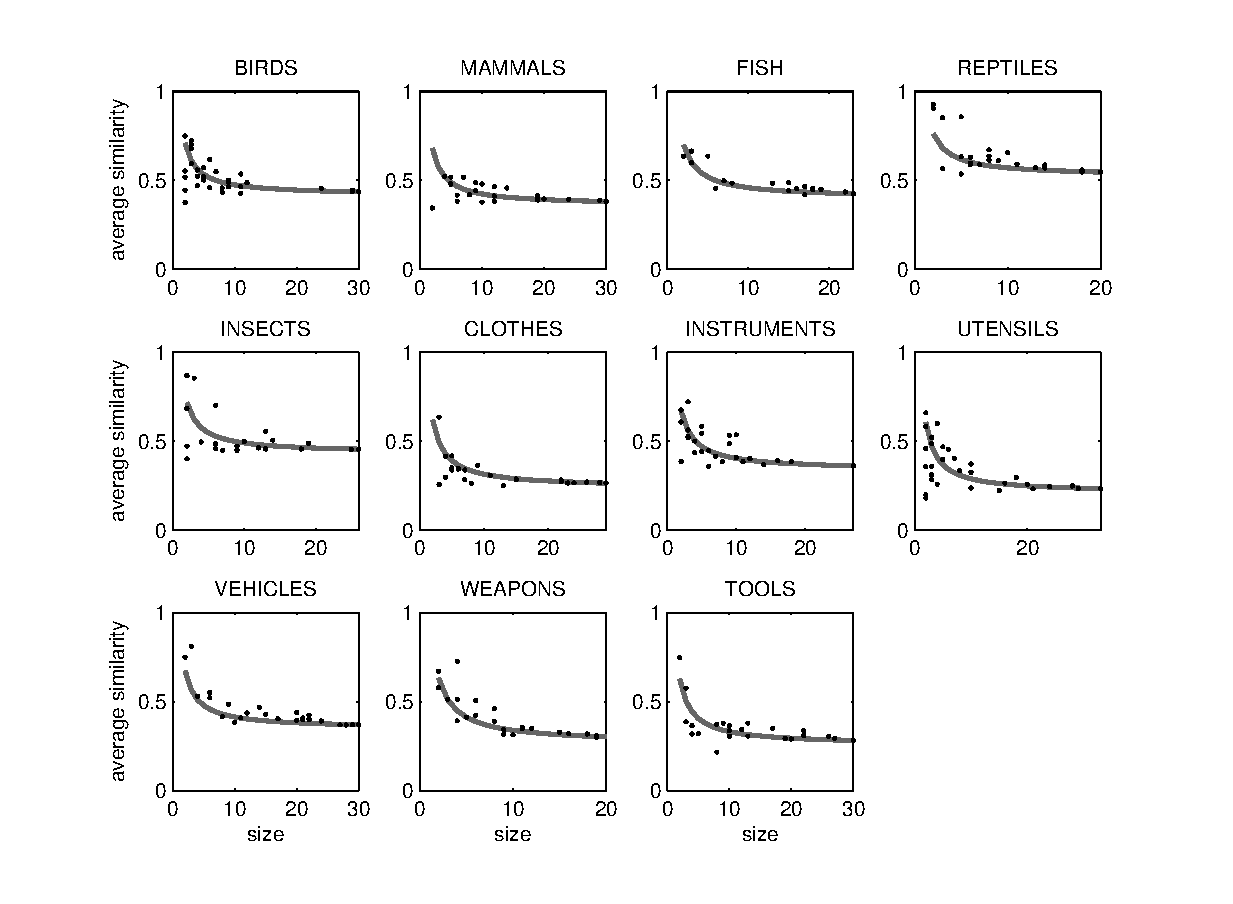
\epsfig{file=sizesim3.eps, width=16cm}
\caption{The average intra-class similarity implied by those features that reached the 3\% cutoff.  Each black dot plots the average {\it similarity} among items with a particular feature ($x$ axis) against the {\it number of items} with the feature ($y$ axis). The solid lines plot the {\it a priori} predicted relationship constructed from the size principle (i.e., Equation~\ref{sizespec}). In most cases (see Table~\ref{modelpost}) this prediction corresponds to the best model for the data.}
\label{sizedata}
\end{center}
\end{figure}



\begin{table}
\begin{center}
\caption{Three types of correlation. Only the significant correlations are listed. In total, 32 of the 33 correlations were significant, strongly suggesting that a relationship exists.}
\label{correls}
\begin{tabular}{l|ccc} \hline dataset & rank-order & linear & inverse \\ \hline
birds      &  {-0.62} & -0.54 & 0.51 \\
mammals    &  -0.49 & {-0.51} & --  \\
fish       &  -0.85 & -0.84 & {0.89} \\
reptiles   &  -0.66 & -0.65 & {0.89} \\
insects    &  -0.32 & -0.42 & {0.48} \\
clothes    &  -0.64 & -0.57 & {0.67} \\
instruments&  {-0.67} & -0.60 & 0.61 \\
utensils   &  -0.53 & {-0.59} & 0.47 \\
vehicles   &  -0.84 & -0.73 & {0.92} \\
weapons    &  {-0.89} & -0.78 & 0.85 \\
tools      &  -0.74 & -0.52 & {0.80} \\
\hline
\end{tabular}
\end{center}
\end{table}



The raw data for our analysis are plotted in Figure~\ref{sizedata}. In each domain, we have a collection of 20--30 high-frequency ($>$3\%) features, and we wish to see if there is a relationship between the number of items that possess the feature $n_k$, and the average similarity $\bar{s}_k$ between pairs of such items. These are the two variables plotted in the figure, with each dot corresponding to a feature, and the solid line showing the specific curve predicted by the size principle (Equation~\ref{sizespec}). Visual inspection suggests that the prediction is consistent with the data: in what follows, we provide a more detailed analysis.

The first analysis we consider is simply to examine the correlations. For all 11 data sets, we calculated Spearman rank-order correlations between $n_k$ and $\bar{s}_k$, as well as the corresponding Pearson linear correlations, and the Pearson correlations between $1/n_k$ and $\bar{s}_k$. As is shown in Table~\ref{correls}, the results are significant in almost all cases.  Given this, we can state with considerable confidence that there exists some monotonic functional relationship between the two variables; but cannot be sure whether the relationship is linear (i.e., $y=-ax+b$), inverse (i.e., $y=a/x+b$) or some other monotonic decreasing function.



In order to obtain some sense of this, we turn to a Bayesian data analysis in which we consider three models. All three models take the form
\begin{equation}
\bar{s}_k = \mu(n_k,\theta) + \epsilon_k,
\end{equation}
\noindent
where $\mu(n_k,\theta)$ is the predicted value for the similarity as a function of the size. In this expression, the error terms $\epsilon$ are assumed to be i.i.d., normally distributed, with mean zero and unknown standard deviation $\sigma$. We set the prior over $\sigma$ in a (weakly) data-dependent way: across all 11 data sets and every possible value of $n_k$ for which we had three or more data points, we took frequentist (i.e., Bessel-corrected) variance estimates, excluding cases with suspiciously low standard deviation (i.e., below 0.01). We then constructed a prior over $\sigma$ by fitting a gamma distribution to these estimates (which provided a reasonably good fit). This yielded a gamma(1.77,0.045) distribution, meaning that the prior expected value of $\sigma$ is 0.08, and a 90\% prior confidence that $\sigma \in [0.01,0.20]$. Given that the data can only fall in the range [0,1], this prior distribution over noise levels seems reasonable.



The mean functions $\mu()$ for the three models are:
\begin{eqnarray}
\mathcal{M}_1, \mbox{constant:} &\mu(n_k,b) =& b \\
\mathcal{M}_2, \mbox{linear:} &\mu(n_k,a,b) =& a(n-n_k)/(n-1) + b \\
\mathcal{M}_3, \mbox{inverse:} &\mu(n_k,a,b) =& a/n_k + b.
\end{eqnarray}
\noindent
In all three cases, we assume normal priors, and for the moment we consider only the prior mean. For all three, the prior mean is over $b$ is fixed at $\bar{s}$, since we expect that as $n \rightarrow \infty$ the intraclass similarity just converges to the domain average. Correspondingly, since $s_{ii}=1$, the prior conditional mean for $a|b$ becomes $1-b$ in both the inverse and linear models (this is the reason for writing the linear model in this odd form: the constraints described in the previous section induce the same prior for both models). For the sake of conservativeness, we set the prior standard deviation fairly large in each case, at 0.2.


Having done so, we numerically approximate the marginal probability of the observed intraclass similarities $\mat{\bar{s}}=[\bar{s}_k]$ for model $\mathcal{M}$,
\begin{equation}
\Pr(\mat{s} \given \mat{n}, \mathcal{M})  = \int_0^\infty \int_\Theta \prod_k \Pr(s_k | n_k, \theta,\sigma) \Pr(\theta|\mathcal{M}) \Pr(\sigma) \ d\theta \ d\sigma,
\end{equation}
where $\mat{n}=[n_k]$ denotes the vector of feature sizes. From this, we can calculate the posterior distribution over models for each data set. The results are shown in Table~\ref{modelpost}. Not surprisingly, they are broadly in agreement with the simpler frequentist analysis in Table~\ref{correls}, but equally unsurprisingly there are some differences. Most strikingly, the inverse model (consistent with the size principle) provides a superior fit to the other models in 9 of 11 cases, and is competitive in the two cases that the linear model wins. Since the Bayesian analysis that we have conducted automatically accounts for model complexity \cite<e.g.,>{Myung1997}, this gives strong evidence that the inverse rule is the right one for these data.

\begin{table}
\begin{center}
\caption{Posterior distribution over three models for the data, reported as pairwise betting odds for the model, relative to the best model in the set. Thus, the winning model is at even odds (i.e., 1:1), whereas a model that is assigned posterior probability of only 1/100th that of the best model is at 100:1. All models that are ``indistinguishable'' from the best model (odds not worse than 20:1, by analogy to the $\alpha=0.05$ standard in null hypothesis testing) are boldfaced.}
\label{modelpost}
\begin{tabular}{l|rrr}  \hline dataset & constant & linear & inverse \\ \hline
birds       &  98.5 & {\bf 3.64} & {\bf 1}   \\
mammals     &  558 & {\bf 1} & {\bf 10.4}    \\
fish        &  $>$1000 & 58.0 & {\bf 1}  \\
reptiles    &  $>$1000 & $>$1000 & {\bf 1} \\
insects     &  {\bf 16.2} & {\bf 4.69} & {\bf 1}   \\
clothes     &  $>$1000 & 123 & {\bf 1}   \\
instruments &  157 & {\bf 4.54} & {\bf 1}    \\
utensils    &  263 & {\bf 1} & {\bf 10.4}    \\
vehicles    &  $>$1000 & $>$1000 & {\bf 1} \\
weapons     &  $>$1000 & 182.3 & {\bf 1} \\
tools       &  $>$1000 & $>$1000 & {\bf 1} \\
\hline
\end{tabular}
\end{center}
\end{table}


\subsection{Possible confounds or artifacts}

At this point there is clear evidence for an inverse feature-size effect in the data. However, before attributing the effect to the operation of a size principle, it is important to consider possible artifactual explanations. In this subsection we evaluate three possibilities: feature-listing frequency, base rate of feature size, and correlated feature assignments.

\begin{figure}
\begin{center}
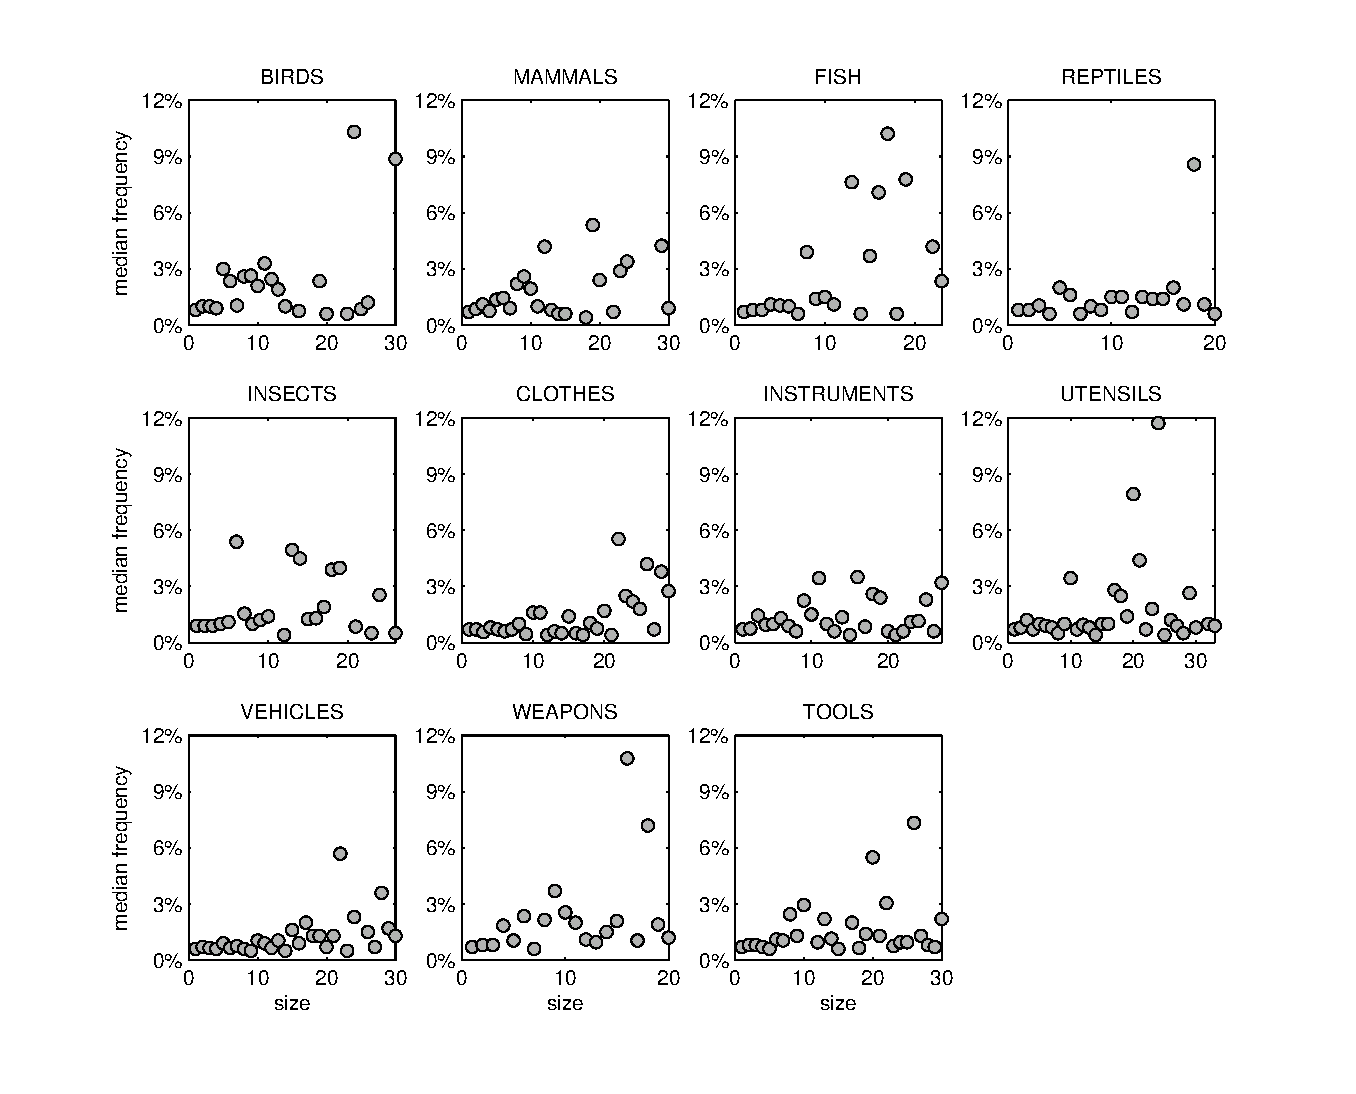
\epsfig{file=featurefreq3.eps, width=16cm}
\caption{Median feature-listing frequency as a function of size. Two data points are not shown: $n$=29, freq=15.05 for the birds data, and $n$=25, freq=23.42 for the insect data. Across the 11 data sets, there is a tendency for larger features to be mentioned slightly more frequently (rank order correlations range from 0.19 to 0.60). Significant correlations are found in the \domain{fish} ($\rho=0.54$), \domain{clothes} ($\rho=0.51$) and \domain{vehicles} ($\rho=0.60$) domains.}
\label{sizegen}
\end{center}
\end{figure}

The first possibility relates to the frequency with which people listed each feature. One might suppose that it is actually high list-frequency features that are strongly weighted, and small features are simply more likely to be listed than are large features. This would still imply a real effect, just not the one we are interested in; however, it does not appear to be the case. Figure~\ref{sizegen}  plots the median feature generation frequency as a function of size for all features, not just those that reached the cutoff. If anything, across the 11 domains, there is a weak tendency for the larger features to be listed with a higher frequency (though only the \domain{mammals} and \domain{fish} data show the effect strongly). Given the lack of any systematic biases, it seems unlikely that the highly consistent size effect in Figure~\ref{sizedata} can be explained in this manner.



\begin{figure}
\begin{center}
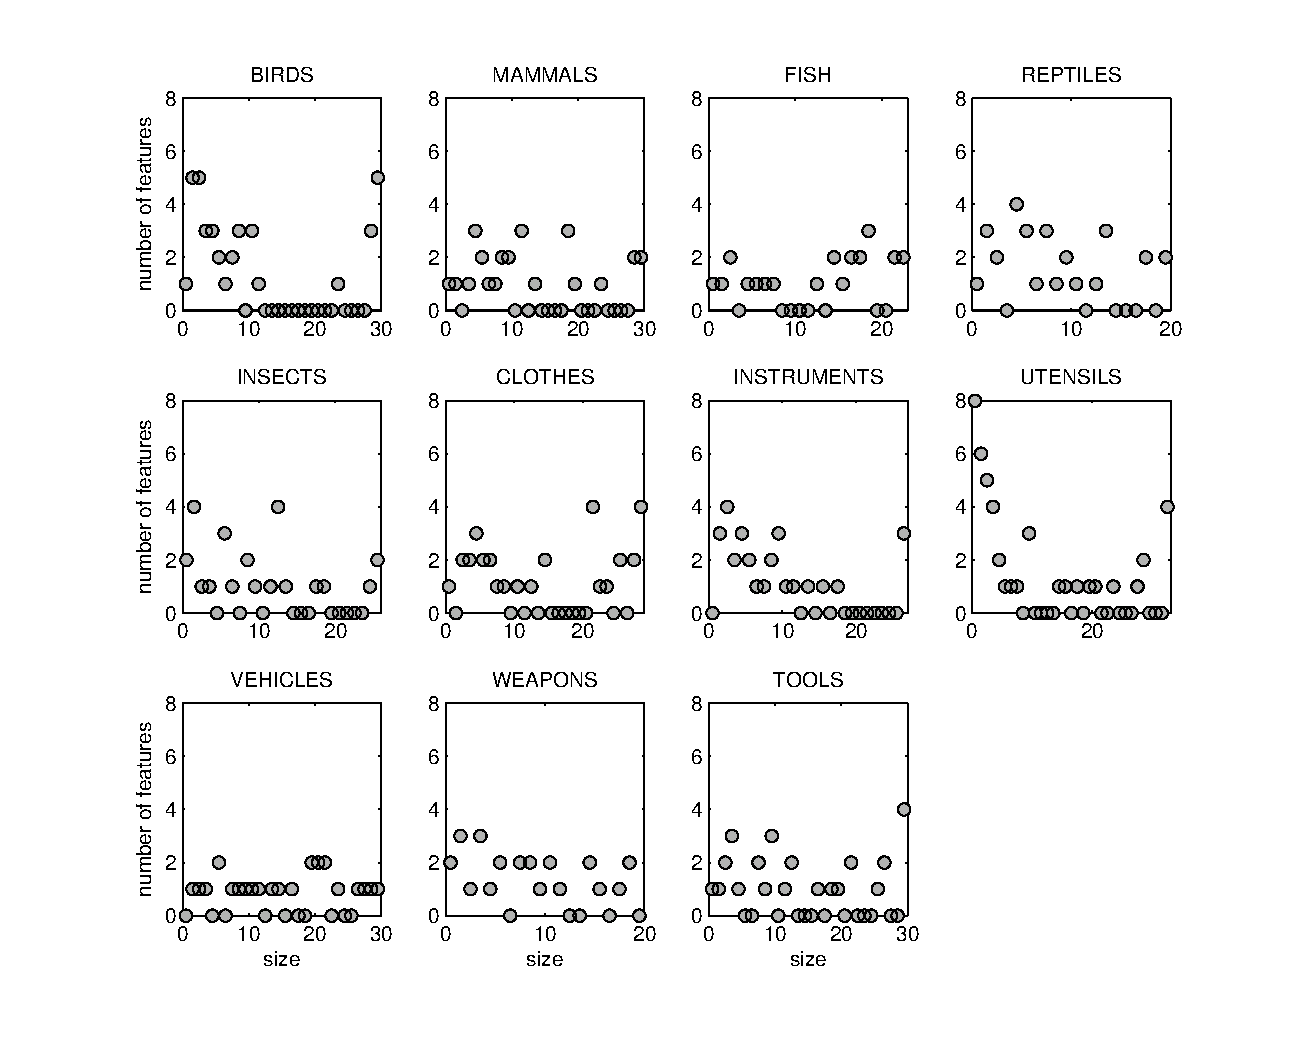
\epsfig{file=featurecounts2.eps, width=16cm}
\caption{The number of features that reach 3\% cutoff, plotted as a function of size. There is a tendency to see more small features in 5 of the data sets: \domain{birds} ($\rho=-0.47$), \domain{insects} ($\rho=-0.39$), \domain{instruments} ($\rho =-0.57$), \domain{utensils} ($\rho=-0.44$) and \domain{weapons} ($\rho=-0.47$), though in some cases (most noticably \domain{birds} and \domain{utensils}) the data are actually asymmetric U-shapes.}
\label{sizeskept}
\end{center}
\end{figure}



A related possibility is that the size effect results from the somewhat arbitrary 3\% cutoff that we imposed. While we do think that it is important to use some cutoff in order to avoid idiosyncratic features that are listed by few people and probably do not form part of the usual mental representations people apply, it is nevertheless essential to check that this does not unfairly influence the results.  How can we be sure that many very small, very unimportant features are not being censored by the 3\% rule, and that {\it this} is the origin of the effect? If this were the case, it would not be an artifact -- it would be a variant on the size principle itself, just expressed in a different fashion \cite<see>{Navarro2009} -- but either way, it is important to check that we have not set the cutoff in such a way as to completely censor features of a particular size (that is, we want to have a similar quantity of data points at different values of $n_k$). To evaluate this, Figure~\ref{sizeskept} shows the total number of features that reach the 3\% threshold as a function of size. The typical pattern across domains is that features that pick out smaller classes tend to be more likely to reach the generation threshold, but this is not universal. Importantly, there is enough variability in feature size within most domains to allow the size effect to emerge, and enough variability between domains to make a consistent size effect less likely to be artifactual.

\begin{figure}
\begin{center}
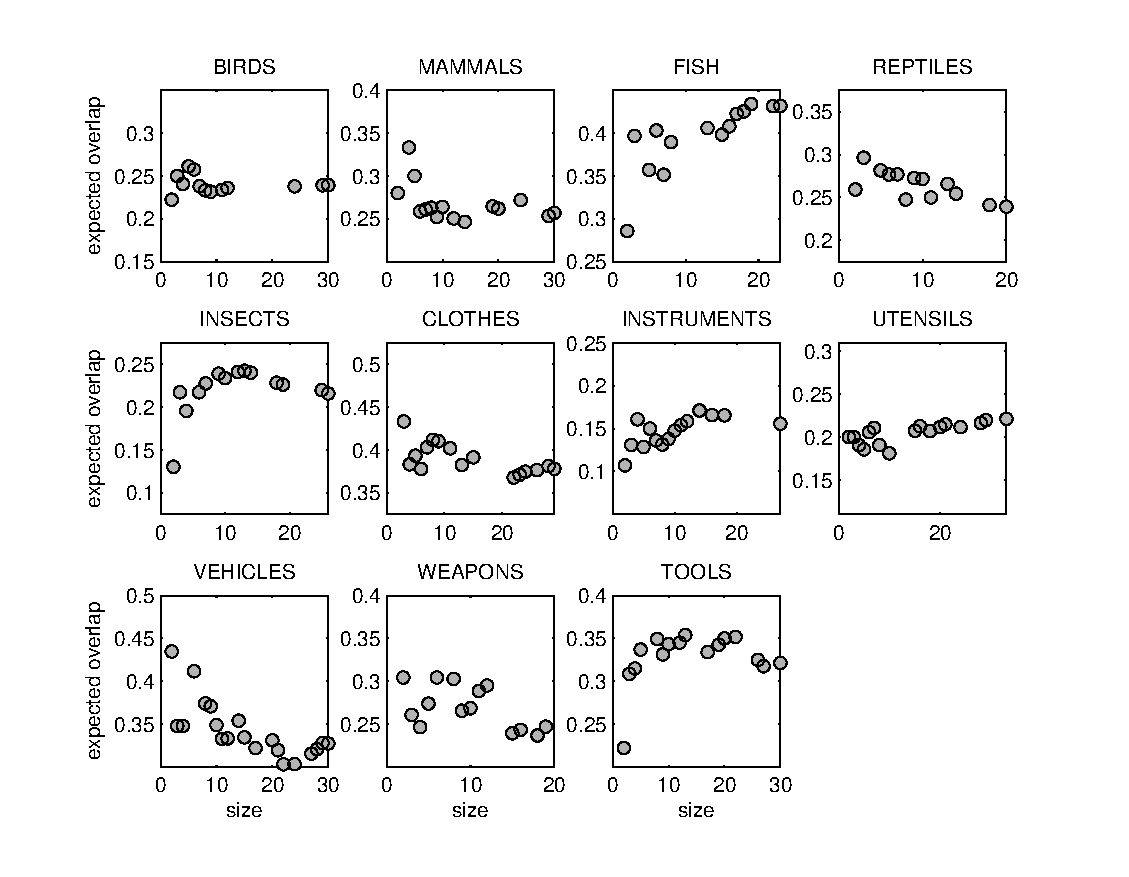
\epsfig{file=overlap.eps, width=16cm}
\caption{The conditional probability that two items will share other features given that they share a feature of size $n_k$. In most cases, there are strong correlations (indicating highly structured features), but the direction of the correlation varies wildly. Significant  positive rank-order correlations exist for \domain{fish}, \domain{insects}, \domain{instruments}  and \domain{utensils} and significant {\it negative} correlations exist for \domain{mammals}, \domain{reptiles}, \domain{clothes}, \domain{vehicles} and \domain{weapons}. No significant relationship exists for either \domain{birds} or \domain{tools}.}
\label{overlap}
\end{center}
\end{figure}

The third potential artifact is the most subtle, and the one about which most care is required. When constructing the size law in Equation~\ref{sizespec}, we made the assumption that the feature assignments were largely independent of one another. In practice, one does not expect this to be true: the feature \feature{has feathers} is extremely closely related to \feature{can fly}, for instance. In and of itself, an incorrect assumption of independence is not too much of a problem, since (as the statistical saying goes) all models are wrong. However, it might be the case that features have a very strong tendency to be nested inside one another (i.e., the set of things that have feathers is (very nearly) nested inside the set of things that fly). If so, then two entities that are known to share a small feature will also {\it necessarily} share all the larger features that it sits inside. The reverse would not be true for two entities known to share a large feature. As a consequence, the number of {\it additional} features that contribute to the pairwise similarity (i.e., number of nonzero terms in the second part of Equation~\ref{splitcf}) would not be independent of $n_k$. If true, this would mean that small features are not highly weighted because they are seen as more important in and of themselves, but because they are correlated with more of the other features in the domain; that it is only due to the combined influence that these other features have on the similarity that the small feature appears to be highly weighted.

Leaving aside the thorny question of whether this would actually count as an artifact,\footnote{One could argue that a heightened correlation with other features is a sign of feature centrality \cite{Sloman1998a} and hence a good measure of internal coherence \cite{Rogers2004}. As a result, one might very well be inclined to treat this as something more than artifact.} it is simple enough to test whether this is the case for these data. Figure~\ref{overlap} plots the conditional probability that, given that two items share a feature of size $n_k$, they will also share other features. In most cases there are strong correlations, indicating highly structured features, but the direction of the correlation varies wildly. Significant ($p<0.05$) positive rank-order correlations exist for \domain{fish} ($\rho=0.91$), \domain{insects} ($\rho=0.53$), \domain{instruments} ($\rho=0.74$) and \domain{utensils} ($\rho=0.62$). However, there are significant negative correlations for \domain{mammals} ($\rho=-0.43$), \domain{reptiles} ($\rho=-0.70$), \domain{clothes} ($\rho=-0.60$), \domain{vehicles} ($\rho=-0.84$) and \domain{weapons} ($\rho=-0.53$). No significant relationship exists for either \domain{birds} or \domain{tools}. Hence, dependencies among the $f_{ik}$ values do not appear to be the source of the effect.


\subsection{Testing the predictions of our derivation}

\begin{figure}
\begin{center}
\hspace*{-2cm}
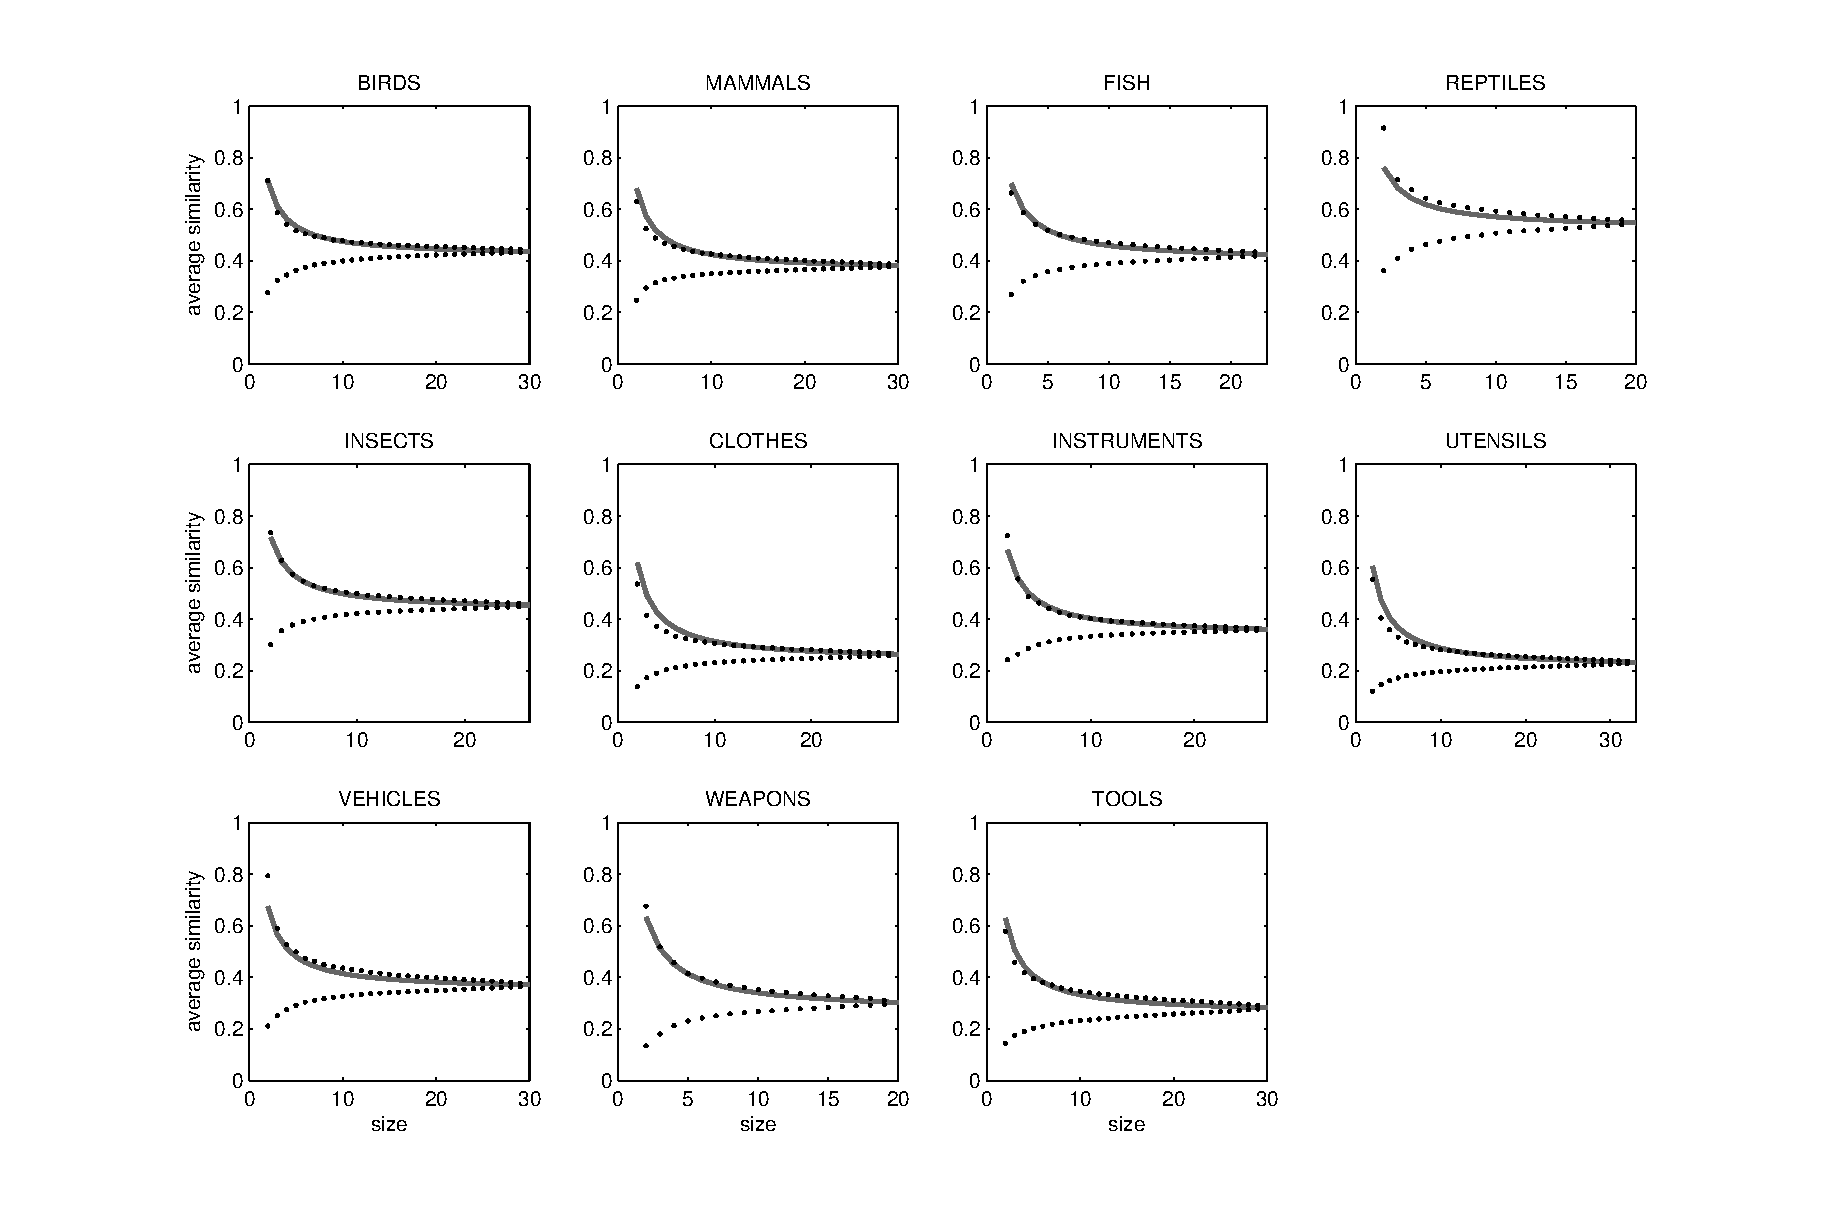
\epsfig{file=sizesim2.eps, width=19cm}
\caption{The 95\% confidence intervals (dotted lines) for a randomly chosen feature as a function of the size of the class of objects picked out by the feature. Note that the upper bound (i.e., the 97.5th percentile of the distribution over intra-class similarities) very closely matches the ``$1/n$'' rule for size-similarity relationships (solid lines).}
\label{awesome}
\end{center}
\end{figure}

In the second part of this paper, we derived an expression for the distribution of intraclass similarities as a function of the number of entities assigned to the class (the size law), and showed that the $y$th percentile of this distribution is given by Equation~\ref{ydist}. How closely does this expression match the actual distribution implied by the Leuven similarity matrices? After all, the real data are much more structured than the minimal case used to derive the $1/n$ law, and may show a different pattern. However, as is shown in Figure~\ref{awesome}, the predicted pattern is almost perfectly reproduced in all 11 subjective similarity matrices. The solid lines plot the size principle predictions (identical to those used in Figure~\ref{sizedata}), while the dotted lines plot bootstrap estimates of the 2.5th and 97.5th percentiles of the empirical distribution over the intraclass similarities among possible subsets of entities, as a function of the size of the subset: for any given feature size, we generated 10000 features at random and calculated the implied intraclass similarity for each. Each black dot marks the 2.5th percentile or 97.5th percentile of these distributions. As expected, the upper percentiles show the ``$1/n$'' effect very strongly for all 11 similarity matrices -- the theoretical Bayesian prediction used in Figures~\ref{sizedata} and~\ref{awesome} is almost indistinguishable from the 97.5th percentile line. This correspondence implies that the size principle may be justifiable in terms of a kind of representational or communicative optimality, in the sense described earlier.

%\subsection{Biases in additive clustering}

Tests of our derivation may extend in other directions too. One of the consequences of treating the size principle as a corollary of feature discovery is that we can draw parallels with additive clustering methods \cite{Shepard1979,Tenenbaum1996,Lee2001a,Navarro2008a} that try to solve the feature discovery problem from a statistical learning perspective. For instance, the original algorithm proposed by \citeA{Shepard1979} to perform inference in the additive clustering model used an ``elevated subsets'' heuristic to pick out clusters of entities with higher internal similarities than any of its supersets. If people adopt a similar strategy, then an optimal solution to the feature generation task would be to list features that are as large as possible without sacrificing too much in terms of internal coherence. With this in mind, a natural prediction of the feature discovery view of the size principle is that additive clustering methods should produce the effect for purely artifactual reasons.
That is, the size principle should emerge when additive clustering models are fit to noisy data, even if there was no inherent size effect in the similarity matrix to begin with.\footnote{This would not prohibit real size effects from existing in human-generated data as well, of course. In fact, in light of the results in this paper it would be odd if there were not real size effects in the data. It is ``just'' that one would need to take care to avoid the confound with the artifactual version.}

As a initial test of this proposition, we generated 100 artificial similarity matrices in domains with 15 entities and 10 features. The cells of the $15 \times 10$ feature matrix were generated as independent Bernoulli draws with underlying rate of 0.3. The saliency attached to each feature was drawn from a uniform distribution on [0.1, 0.4], and then added independent zero-mean Gaussian noise was added with $\sigma =0.15$, corresponding to moderately noisy data. We then ran the Bayesian additive clustering algorithm proposed by \citeA{Navarro2008a} on the data, using a more diffuse hierarchical prior than the one in the original paper.\footnote{The choice to use the hierarchical prior (on the $\alpha$ parameter for the Indian buffet process used in that paper) was deliberate -- by maximizing the uncertainty associated with the model, the posterior distribution over $(\mat{F},\mat{w})$ includes a lot of cases of overfitting, {\it and} lots of cases of underfitting. The result is a simulation designed to exaggerate the bias -- the extent to which this is a serious bias in normal uses of additive clustering remains unknown.}
While the complete details of the feature recovery are not of immediate interest, the key effect is the weak but significant tendency for the {\it error terms} in the estimated weight to be non-uniform as a function of size ($\rho=-0.13$, $p=6.3\times10^{-5}$), as illustrated in Figure~\ref{artifact}. As predicted, the estimated weights of recovered features are biased upwards if the features are small. Why does this happen? Although additive clustering does not explicitly seek to include all features that meet some analytically-specified criterion (as we did in our empirical analysis), it is nevertheless a statistical learning tool designed to determine whether or not different groups of stimuli are sufficiently similar to one another to be worth positing the existence of a feature. As such, it may be deemed to adopt an implicit criterion. Since small features contribute to fewer cells in $\mat{S}$, the implicit criterion for inclusion necessarily shifts upwards. Or, to put it another way, there is a size by weight interaction effect when predicting additive clustering's ability to extract a feature from data (rank-order correlation with the interaction term is $\rho = 0.35$, $p = 1.1\times10^{-30}$, after controlling for main effects): if a proposed feature is small and low-weight, it is unlikely to be acceptable to the additive clustering algorithm, for the exact same reason that we argue that it is unlikely to be acceptable to people.


\begin{figure}[t]
\begin{center}
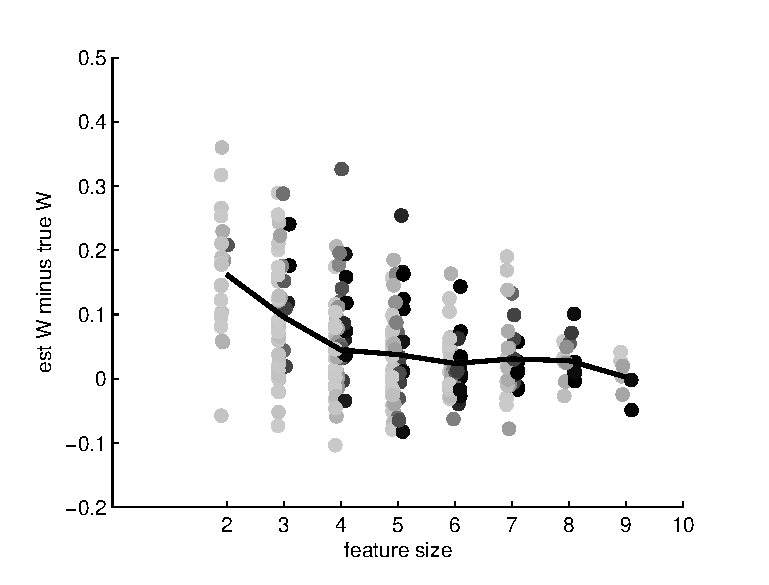
\epsfig{file=theartifact.eps,width=8cm}
\caption{An ``artifactual'' size law in additive clustering: when learning features from noisy data, small low-weight features are differentially more likely to be censored from the learned representation, leading to a correlation between size and average estimated weight. The differently colored dots denote features with different recovery probability: dark dots denote features recovered with high probability, while light dots denote features that are rarely successfully recovered.}
\label{artifact}
\end{center}
\end{figure}

\section{Conclusion}

We have demonstrated that the ``size principle'' for featural similarity previously derived based on  sampling assumptions is also explainable on the basis of communicative or representational optimality. A rational agent who seeks to include only those features which are coherent -- i.e., those features for which the objects with those features are highly similar -- will prefer features that describe only a small number of objects. Moreover, the weight of this preference will scale according to a $1/n$ law, where $n$ is the number of objects that possess the feature. We tested this prediction on 11 different datasets in two different domains, and found that human judgments are broadly in agreement with this law. Potential confounds and artifacts were evaluated and rejected.

There are a number of potential extensions to this work. Following a suggestion made by \citeA{Tenenbaum2001}, we might consider the human similarity data alone (without using the listed features), and examine whether the latent features extracted by additive clustering methods satisfy the $1/n$ law. With recent advances in additive clustering methods \cite{Navarro2008a} this approach may be feasible, but a great deal of care would be required to control for the effect shown in Figure~\ref{artifact}. In the more immediate context of considering the relationship between similarity and listed features, one possibility would be to use more sophisticated feature selection methods than the 3\% cutoff used here \cite<e.g.,>{Zeigenfuse2009}, though the artifact may exist in these cases too. It would also make sense to explore data sets that extend beyond the domains of \domain{animals} and \domain{artifacts} to see if the rule holds more generally.

For now, the fact that the Bayesian theory of generalization proposed by \citeA{Tenenbaum2001} predicts the exact same pattern as the one we have derived via the central limit theorem seems unlikely to be a coincidence. Both lead to $1/n$ rules and both carry a strong suggestion of optimal statistical inference. In one sense, the explanations are distinct -- the original theory of generalization treats the feature set as fixed and looks at what constraints apply to optimal similarity judgment, while our analysis examines the constraints that apply to optimal feature discovery and selection when the world (or the learner) provides a similarity structure to encode. If features are given to the learner, they impose a $1/n$ law on similarities, and if similarities are given they impose a $1/n$ law on features. In both cases, the law is an expression of fundamental statistical rules, and it appears to be a strong, elegant regularity in human judgments.

\section{Acknowledgements}

DJN was supported by an Australian Research Fellowship (ARC grant DP0773794). We would like to thank Nancy Briggs, Matt Dry, Tom Griffiths, Michael Lee, Josh Tenenbaum, Rachel Stephens and the reviewers for many helpful comments, discussions and correspondence that greatly improved this article; and Toby Elmhirst for his suggestion about how to use the word ``poppycock.'' Finally, we would like to thank Gert Storms for organizing the workshop and the Belgian National Science Foundation for their support of the workshop.

%\setlength{\baselineskip}{12pt}
%\setlength{\bibleftmargin}{1.5em}
%\setlength{\bibindent}{-1.5em}
%\setlength{\bibitemsep}{0pt}
%\bibliographystyle{apacite}
%\renewcommand{\bibliographytypesize}{\small}
\bibliography{djn}

\end{document}
